\begin{filecontents*}{document.bib}
@article{gerhardt2011,
  title={Experimentally Faking the Violation of Bell’s Inequalities},
  author={Gerhardt, Ilja and Liu, Qin and Lamas-Linares, Ant{\'\i}a and Skaar, Johannes and Scarani, Valerio and Makarov, Vadim and Kurtsiefer, Christian},
  journal={Physical Review Letters},
  volume={107},
  number={17},
  pages={170404},
  year={2011},
  publisher={APS}
}
@article{bell1964,
  title={On the Einstein Podolsky Rosen Paradox},
  author={Bell, John S},
  journal={Physics Physique Fizika},
  volume={1},
  number={3},
  pages={195},
  year={1964}
}
@article{vonneumann1951,
  title={Various techniques used in connection with random digits},
  author={Von Neumann, John},
  journal={National Bureau of Standards Applied Math Series},
  volume={12},
  pages={36--38},
  year={1951}
}
@article{shor2000,
  title={Simple proof of security of the BB84 quantum key distribution protocol},
  author={Shor, Peter W and Preskill, John},
  journal={Physical Review Letters},
  volume={85},
  number={2},
  pages={441},
  year={2000}
}
\end{filecontents*}

\documentclass[12pt,twocolumn,letterpaper,english]{article}

% --- Packages ---
\usepackage[T1]{fontenc}
\usepackage[utf8]{inputenc} 
\usepackage[margin=1.75cm,columnsep=0.75cm,headheight=26pt,includeheadfoot]{geometry}
\usepackage[english]{babel}
\usepackage{listings}
\usepackage{color}
\usepackage{titlesec}
\usepackage{titling}
\usepackage{changepage}
\usepackage{amsmath}
\usepackage[colorlinks=true, linkcolor=red, urlcolor=blue, citecolor=blue]{hyperref}
\usepackage{enumitem}
\usepackage{graphicx}
\usepackage{fancyhdr}
\usepackage{lastpage}
\usepackage{caption}
\usepackage{tocloft}
\usepackage{setspace}
\usepackage{multirow}
\usepackage{float}
\usepackage{booktabs}
\usepackage{indentfirst}
\usepackage{xcolor}
\usepackage{csquotes}
\usepackage{amssymb}
\usepackage{pdfpages}

% --- Custom Formatting ---
\newcommand{\Title}{Device-Independent Quantum Communication Technology: From Theory to Hardware Security}
\title{\Title}
\author{Prince Kumar (230051013)}

\pagestyle{fancy}
\fancyhf{}
\lhead{Seminar Progress Report}
\rhead{Prince Kumar (230051013)}
\cfoot{\thepage}

\titleformat{\section}{\large\bfseries\sffamily\raggedright}{\thesection}{1em}{}
\titleformat{\subsection}{\normalsize\bfseries\sffamily\raggedright}{\thesubsection}{1em}{}

\begin{document}


% ==========================================
% PLAGIARISM REPORT
% ==========================================
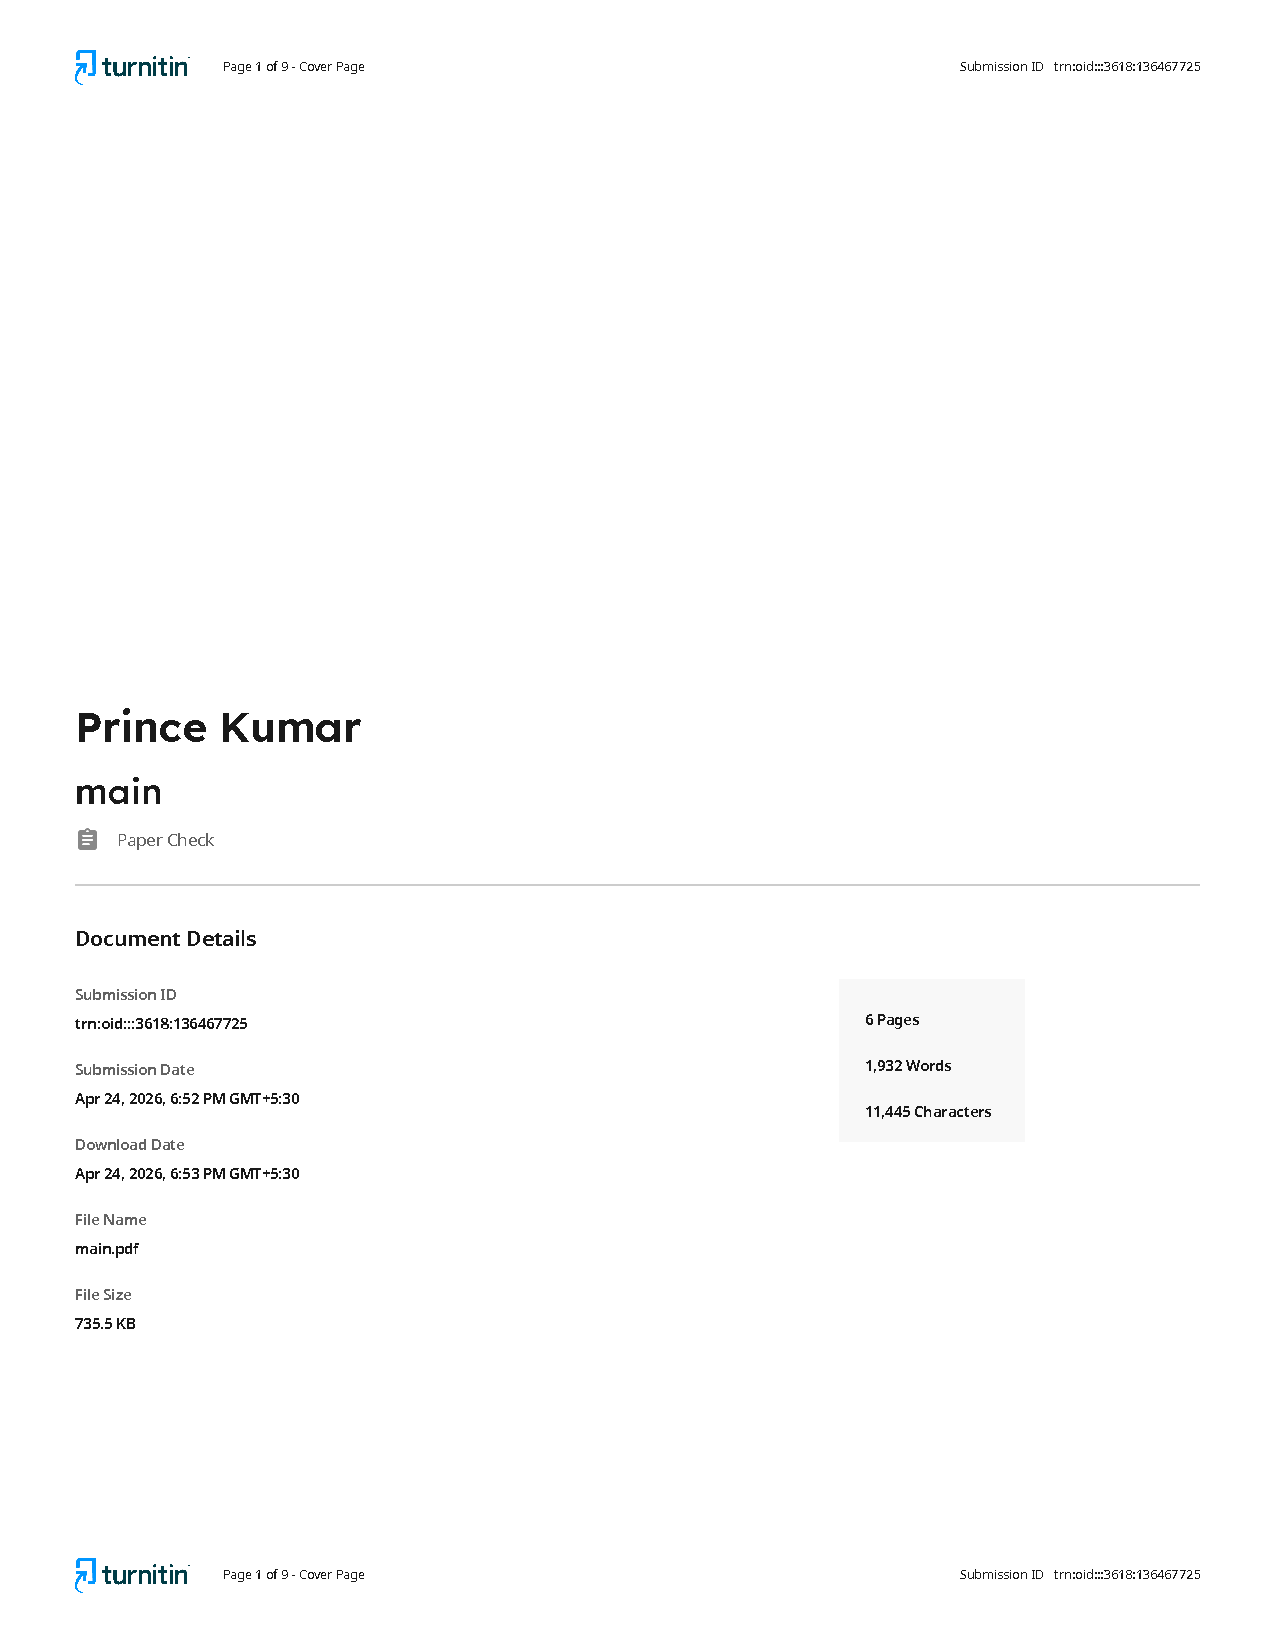
\includepdf[pages={1-3}]{plagarism-report.pdf}

% ==========================================
% TITLE PAGE
% ==========================================
\begin{titlepage}
\begin{center}
\vspace{1cm}

\includegraphics[scale=0.1]{root/IITI_Logo.png}~\\[1cm]
{\LARGE\bf B.Tech. Engineering Physics}\\[0.5cm]
{\Large Seminar Progress Report}\\[2cm]

\hrule
\vspace{.5cm}
{\huge \bfseries \Title} \\ [0.4cm]
{\Large \bfseries Quantum Information \& Cryptography} 
\vspace{.5cm}
\hrule

\vspace{2cm}
\textsc{\textbf{Author}}\\
\vspace{.5cm}
{\large\bf Prince Kumar (230051013)} \\

\vspace{1.5cm}
\textsc{\textbf{Advisor}}\\
\vspace{.5cm}
{\large\bf Dr. Shashank Gupta} \\

\vfill
{\large \today}
\end{center}
\end{titlepage}

\pagenumbering{arabic}
% Line spacing set to default single spacing for dense, academic two-column format.

% ==========================================
% ABSTRACT
% ==========================================
\section*{Abstract}
\addcontentsline{toc}{section}{Abstract}
Quantum Key Distribution (QKD) promises information-theoretic security guaranteed by the laws of quantum mechanics. However, practical implementations rely on physical hardware that introduces critical security loopholes. This report details the theoretical foundations of quantum entanglement, the physical architecture of entanglement-based QKD networks, and the specific hardware vulnerabilities present in Avalanche Photodiodes (APDs). By analyzing a known detector-blinding exploit that perfectly fakes a Bell inequality violation (scoring an unphysical $S = 2.797$), this report demonstrates the necessity of Device-Independent QKD (DI-QKD). Furthermore, because DI-QKD relies entirely on the unpredictability of measurement bases, this report examines Quantum Random Number Generators (QRNGs) and the Von Neumann extraction algorithms required to mitigate secondary hardware biases, ultimately establishing a true zero-trust cryptographic architecture.

% ==========================================
% 1. INTRODUCTION
% ==========================================
\section{Introduction}
Traditional cryptographic protocols rely on computational complexity, rendering them vulnerable to future quantum algorithms like Shor’s algorithm. Quantum Key Distribution (QKD) solves this by leveraging the No-Cloning Theorem and wave-function collapse to provide unconditional security. In a standard QKD model (such as BB84 or BBM92), the quantum channel is mathematically secure; any eavesdropper (Eve) attempting to intercept the flying qubits will inevitably introduce a detectable Quantum Bit Error Rate (QBER).

However, mathematical security proofs often assume the physical hardware—lasers, modulators, and detectors—behaves ideally. In practice, long-distance transmission is severely degraded by exponential fiber loss ($\alpha \approx 0.2$ dB/km) and environmental noise. These physical limitations create a gap between pure theory and optical execution. This report investigates how eavesdroppers exploit this gap at the physical layer, forcing a paradigm shift toward Device-Independent Quantum Cryptography.

% ==========================================
% 2. THEORETICAL FOUNDATIONS
% ==========================================
\section{Theoretical Foundations: The EPR Paradox and Bell’s Theorem}
The development of DI-QKD is deeply rooted in the foundational debates of quantum mechanics, specifically the 1935 Einstein-Podolsky-Rosen (EPR) Paradox.

\subsection{Local Realism vs. Superposition}
Einstein challenged the completeness of quantum mechanics by advocating for "Local Realism." According to EPR, if two particles are entangled, measuring one instantly predicts the state of the other. To avoid "spooky action at a distance" (violating Locality), EPR argued that particles must carry pre-existing instructions or "Hidden Variables" (Realism).

\subsection{The CHSH Inequality}
In 1964, John Bell formulated a mathematical theorem to test Local Realism. The CHSH inequality tests the correlation between measurements made by two parties (Alice and Bob) at varying angles. If the universe operates on classical Hidden Variables, the correlation score ($S$) is strictly bounded: $S \le 2$. 

However, evaluating a maximally entangled Bell state, such as $|\Phi^{+}\rangle = \frac{1}{\sqrt{2}}(|HH\rangle+|VV\rangle)$, yields Tsirelson's bound of $S = 2 \sqrt{2} \approx 2.828$ \cite{bell1964}. This violation proves that particles do not carry pre-determined states, and measurement actively defines reality. 

% ==========================================
% 3. SECURITY PROOF FRAMEWORK
% ==========================================
\section{The Entanglement Security Framework}
To translate entanglement into a secure cryptographic key, systems rely on rigorous mathematical proofs. Figure \ref{fig:bbm92} illustrates the physical layout of the BBM92 protocol, which utilizes an untrusted central source (Charlie).

\begin{figure}[H]
    \centering
    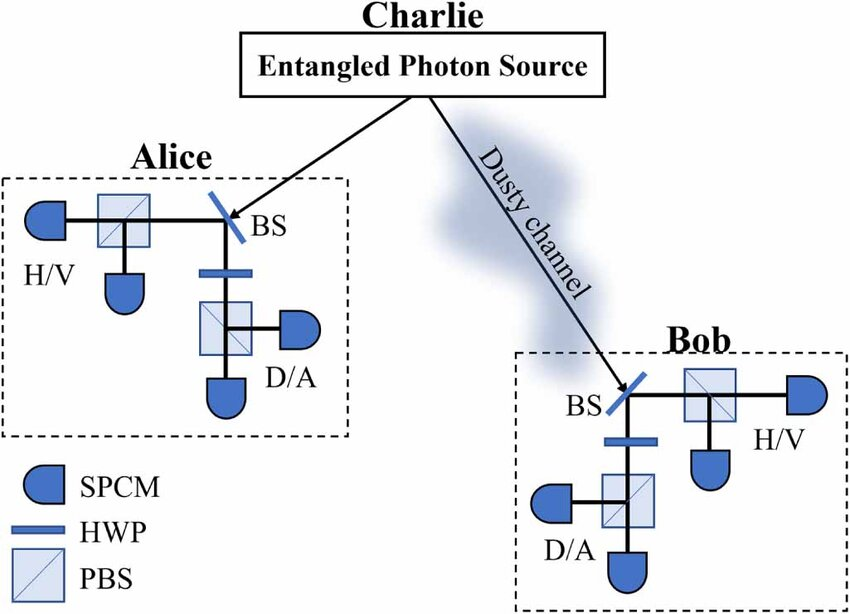
\includegraphics[width=\linewidth]{figures/bbm92.png}
    \caption{The BBM92 Entanglement-Based architecture. An untrusted source (Charlie) distributes photons through a noisy ("dusty") channel to Alice and Bob, who measure in random bases (H/V and D/A) \cite{bbm92_diagram}.}
    \label{fig:bbm92}
\end{figure}

The overarching Shor-Preskill security proof for such a network follows three distinct steps \cite{shor2000}:
\begin{enumerate}
    \item \textbf{Model the quantum state} shared by Alice, Bob, and Eve after the photon traverses the "dusty" channel, but before measurement.
    \item \textbf{Use the observed error rate} (QBER) and entropic inequalities to bound Eve's maximum possible information.
    \item \textbf{Apply classical error correction} and privacy amplification to extract a shorter key about which Eve has negligible information.
\end{enumerate}
The fundamental vulnerability of standard QKD lies in Step 1: if the physical detection hardware (the SPCMs shown in Fig. \ref{fig:bbm92}) is compromised, the mathematical model of the quantum state becomes physically invalid, collapsing the entire security proof.

% ==========================================
% 4. PHYSICAL ARCHITECTURE
% ==========================================
\section{Physical Architecture of Quantum Communication}
To implement these protocols, theoretical states must be engineered into physical photons. Entanglement-based QKD requires highly precise Polarization Entangled Photon Sources (PEPS).

\subsection{The Entanglement Generation Process}
State-of-the-art photon sources utilize a rigorous four-step optical engineering process:

\begin{figure}[H]
    \centering
    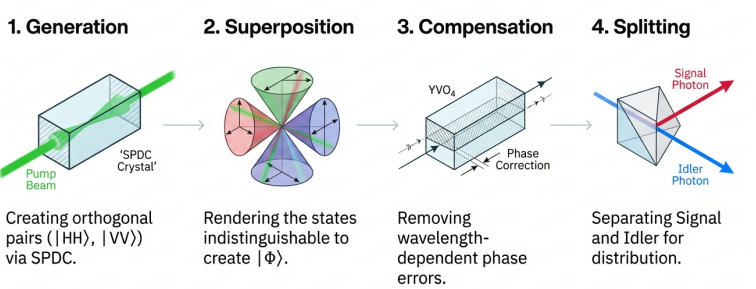
\includegraphics[width=\linewidth]{figures/generation.png}
    \caption{The 4-Step generation process for Entangled Photon Pairs.}
    \label{fig:generation}
\end{figure}

\begin{itemize}
    \item \textbf{Generation:} A high-frequency pump laser drives a non-linear crystal (e.g., BBO or ppKTP), causing Spontaneous Parametric Down-Conversion (SPDC) to create orthogonal pairs.
    \item \textbf{Superposition:} The emission paths are perfectly overlapped to erase "which-path" information, rendering the states indistinguishable.
    \item \textbf{Compensation:} Birefringent crystals (like $YVO_4$) or pre-compensation delay lines are utilized to remove wavelength-dependent phase errors.
    \item \textbf{Splitting:} The paired signal and idler photons are separated via dichroic or wedge mirrors for network distribution.
\end{itemize}

\subsection{Advanced Source Designs}
Modern deployments utilize specific architectures to overcome physical limits. The \textbf{PACES} (Parallel Axis Crystal Entangled Source) design utilizes a half-wave plate sandwiched between BBO crystals, achieving extreme ruggedness proven aboard the SpooQy-1 CubeSat. Alternatively, \textbf{Parallel Path} designs utilize pre-compensation loops to unlock the use of high-power, broadband lasers ($1W+$), which is critical for generating the massive photon flux required to overcome exponential fiber loss.

% ==========================================
% 5. HARDWARE VULNERABILITIES
% ==========================================
\section{Hardware Vulnerabilities: The Detection Loophole}
While the quantum channel is protected by the No-Cloning Theorem, the physical endpoints—specifically the Avalanche Photodiodes (APDs)—are highly vulnerable to optical engineering attacks.

\subsection{Baseline Flaws: Coincidence and PNS}
Physical implementation relies on strict coincidence windows ($t_c \approx 1-2$ ns). Any dark counts or environmental noise registering within this window raises the QBER. If the QBER exceeds the $\approx 11\%$ Shor-Preskill threshold, no secure key can be extracted \cite{shor2000}. Furthermore, because standard lasers follow a Poisson distribution, they occasionally emit multi-photon pulses, allowing Eve to execute a Photon Number Splitting (PNS) attack by capturing the extra photon.

\subsection{The APD Blinding Exploit (Gerhardt et al.)}
A critical vulnerability arises from the physical recovery time of the APDs. Gerhardt et al. demonstrated that an eavesdropper can exploit this by utilizing a Faked-State Generator (FSG) \cite{gerhardt2011}.

\begin{figure}[H]
    \centering
    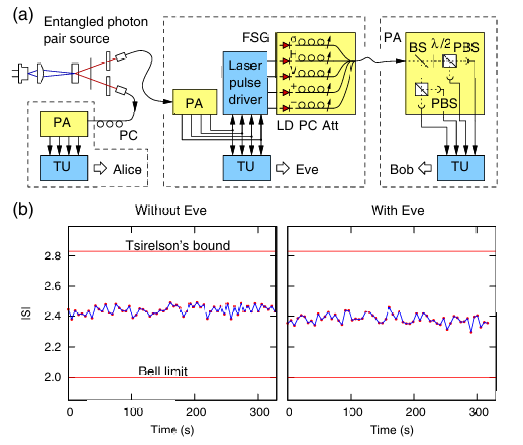
\includegraphics[width=\linewidth]{figures/faking_bell.png}
    \caption{Experimental setup of the faked-state generator intercept-resend attack.}
    \label{fig:faking_bell}
\end{figure}

The attack operates in two phases:
\begin{itemize}
    \item \textbf{Blinding:} Eve shines a continuous, bright, circularly polarized classical laser ($\sigma$) into the receiver. This overloads the APDs, dropping them below the breakdown voltage and pulling them out of Geiger mode, rendering them blind to single photons.
    \item \textbf{Faking the Violation:} Eve intercepts the genuine quantum state, measures it, and fires a tailored, high-intensity linearly polarized classical pulse. This macroscopic pulse forces the targeted blinded APD's current over the threshold, simulating a click.
\end{itemize}

Through this intercept-resend attack, Eve programs the hardware to simulate unphysical correlations. In a passive-choice scheme, this attack achieves 100\% efficiency. In an active-choice setup, it yielded an unphysical correlation score of $S = 2.7971 \pm 0.0005$ with 50\% efficiency \cite{gerhardt2011}. Because the detection efficiency drops, Alice and Bob assume the missing photons were simply lost in transit (the Fair Sampling Assumption), remaining completely unaware of the intrusion.

\subsection{Countermeasures Against Blinding Attacks}
To prevent such faked violations of Bell inequalities using high-energy classical lasers, physical countermeasures can be implemented at the detection endpoints. The most direct defense involves integrating an optical power meter or a dedicated watchdog detector at the receiver's entrance. This watchdog continuously monitors the incoming optical power. If the incident light exceeds the threshold expected for single-photon operations, the system immediately flags the presence of a blinding laser and aborts the key distribution. However, adding physical countermeasures often leads to an "arms race" between new quantum hacking techniques and corresponding hardware patches.

% ==========================================
% 6. DI-QKD
% ==========================================
\section{The Solution: Device-Independent QKD (DI-QKD)}
The hardware exploits demonstrate that attempting to physically secure the endpoints is a fundamentally flawed approach. 

DI-QKD bypasses physical vulnerabilities by treating all equipment as untrusted "black boxes." The mathematical security proof is altered: rather than modeling the quantum state based on the trusted dimensions of the APDs, Alice and Bob use the CHSH Bell test directly on the hardware. 

If the black boxes produce a CHSH score that genuinely violates the classical limit ($S > 2$) with sufficiently high efficiency (closing the detection loophole), the connection is secure. This relies on the \textbf{Monogamy of Entanglement}: if Alice and Bob's particles are maximally entangled, it is mathematically impossible for a third system (Eve) to be correlated with them. If Eve attempts to wiretap the line or fake the states, the CHSH score crashes below the quantum threshold.

% ==========================================
% 7. QRNG PART
% ==========================================
\section{Closing the Loophole: Quantum Random Number Generators}
DI-QKD is fundamentally reliant on the unpredictability of measurement bases. Classical pseudo-random number generators (PRNGs) are algorithmic and deterministic. If Eve can predict the basis choices, she can pre-program the faked states to pass the Bell test. Therefore, true Quantum Random Number Generators (QRNGs) are mandatory.

\subsection{Beam Splitter Architecture}
The foundational QRNG design utilizes a single photon fired at a 50/50 beam splitter. The photon enters a state of spatial superposition and collapses into one of two detectors upon measurement, generating a perfectly random `0` or `1`. Because the outcome does not exist prior to measurement, it cannot be predicted.

\subsection{Hardware Bias and the Von Neumann Extractor}
Like QKD setups, QRNGs are physical devices susceptible to manufacturing defects. An imperfect beam splitter (e.g., transmitting 52\% and reflecting 48\%) yields a statistically biased sequence. 

To counteract this, the raw quantum data is processed through a Von Neumann Extractor \cite{vonneumann1951}. By reading bits in non-overlapping pairs, discarding matching pairs (`00`, `11`), and mapping mixed pairs (`01` $\to$ 0, `10` $\to$ 1), the algorithm mathematically guarantees an unbiased 50/50 distribution, ensuring physical defects do not compromise the overarching DI-QKD protocol. An interactive visualization of this bias elimination process can be found in the accompanying simulation done as a part of this work: \href{https://princekumarofficial.github.io/rng-von-neumann-extractor/}{https://princekumarofficial.github.io/rng-von-neumann-extractor/} \cite{rng_simulation}.

% ==========================================
% 8. CONCLUSION
% ==========================================
\section{Conclusion}
The transition from standard QKD to Device-Independent QKD represents a fundamental shift in cryptographic trust. By acknowledging that physical hardware—from APDs to beam splitters—will inherently possess vulnerabilities, DI-QKD leverages the deepest principles of quantum mechanics to verify security. Through rigorous Bell inequality analysis and the implementation of bias-extracted QRNGs, it is possible to build a communication network that remains completely secure, even when the physical devices operating it have been fundamentally compromised by an adversary.

\newpage
\addcontentsline{toc}{section}{References}
\begin{thebibliography}{10}

\bibitem{bell1964}
J.~S. Bell,
\newblock ``On the Einstein Podolsky Rosen Paradox,''
\newblock \emph{Physics Physique Fizika}, vol.~1, no.~3, p.~195, 1964.

\bibitem{shor2000}
P.~W. Shor and J.~Preskill,
\newblock ``Simple proof of security of the BB84 quantum key distribution protocol,''
\newblock \emph{Physical Review Letters}, vol.~85, no.~2, p.~441, 2000.

\bibitem{gerhardt2011}
I.~Gerhardt, Q.~Liu, A.~Lamas-Linares, J.~Skaar, V.~Scarani, V.~Makarov, and C.~Kurtsiefer,
\newblock ``Experimentally Faking the Violation of Bell’s Inequalities,''
\newblock \emph{Physical Review Letters}, vol.~107, no.~17, p.~170404, 2011.

\bibitem{vonneumann1951}
J.~Von Neumann,
\newblock ``Various techniques used in connection with random digits,''
\newblock \emph{National Bureau of Standards Applied Math Series}, vol.~12, pp.~36--38, 1951.

\bibitem{bbm92_diagram}
ResearchGate,
\newblock ``The block diagram of implemented BBM92 protocol,''
\newblock \url{https://www.researchgate.net/figure/The-block-diagram-of-implemented-BBM92-protocol-HWP-half-wave-plate-PBS-polarizing_fig1_360556529}.

\bibitem{rng_simulation}
Prince Kumar,
\newblock ``Von Neumann Extractor Simulation,''
\newblock \url{https://princekumarofficial.github.io/rng-von-neumann-extractor/}.

\end{thebibliography}

\end{document}